% Pi Coding Agent vertical tutorial PDF header.
% Rendered with Pandoc + XeLaTeX.

\usepackage{fontspec}
\usepackage{xcolor}
\usepackage{tikz}
\usetikzlibrary{arrows.meta,positioning,calc}
\usepackage{etoolbox}
\usepackage{geometry}
\usepackage{titlesec}
\usepackage{fancyhdr}
\usepackage{microtype}
\usepackage{enumitem}
\usepackage{booktabs}
\usepackage{longtable}
\usepackage{array}
\usepackage{framed}
\usepackage{hyperref}

% Keep the visual language aligned with the tutorial decks.
\definecolor{piaccent}{HTML}{D77600}
\definecolor{piblue}{HTML}{4A90D9}
\definecolor{pimut}{HTML}{60605E}
\definecolor{piblack}{HTML}{0A0A0A}
\definecolor{pibody}{HTML}{242424}
\definecolor{picode}{HTML}{F3F0EB}
\definecolor{piline}{HTML}{DDD7CE}

\geometry{
  paperwidth=8.27in,
  paperheight=11.69in,
  top=0.78in,
  bottom=0.72in,
  inner=0.86in,
  outer=0.72in,
  headheight=15pt,
  headsep=0.18in,
  footskip=0.36in
}

\setmainfont{PT Sans}
\setsansfont{PT Sans}
\setmonofont{Andale Mono}[Scale=MatchLowercase]
% Display face for cover + part dividers (matches the Marp deck body,
% which uses STIX Two Text with weight 600 for headings).
% Loaded from the TeX Live static instances by file: the macOS system copy
% is a variable font that XeLaTeX cannot resolve by family name alone.
\newfontfamily\displayfont{STIXTwoText-Regular}[
  Extension=.otf,
  UprightFont=STIXTwoText-Regular,
  BoldFont=STIXTwoText-SemiBold,
  ItalicFont=STIXTwoText-Italic,
  BoldItalicFont=STIXTwoText-SemiBoldItalic
]
\renewcommand{\familydefault}{\sfdefault}
\makeatletter
\renewcommand\normalsize{\@setfontsize\normalsize{11}{14}}
\renewcommand\small{\@setfontsize\small{10}{12.5}}
\makeatother
\AtBeginDocument{\normalsize}
\setlength{\parindent}{0pt}
\setlength{\parskip}{0.6em}
\linespread{1.12}
\emergencystretch=2em
\clubpenalty=10000
\widowpenalty=10000
\setlength{\tabcolsep}{7pt}
\renewcommand{\arraystretch}{1.18}

\hypersetup{
  colorlinks=true,
  linkcolor=piaccent,
  urlcolor=piaccent,
  citecolor=piaccent,
  pdftitle={Pi Agent},
  pdfauthor={Julius Darang}
}

% Headings: restrained, orange chapter markers, no oversized slide typography.
\titleformat{\section}
  {\Large\sffamily\bfseries\color{piaccent}}
  {}{0pt}{}
\titleformat{\subsection}
  {\large\sffamily\bfseries\color{piaccent}}
  {}{0pt}{}
\titleformat{\subsubsection}
  {\normalsize\sffamily\bfseries\color{pibody}}
  {}{0pt}{}
\titlespacing*{\section}{0pt}{2.6em}{0.75em}
\titlespacing*{\subsection}{0pt}{1.7em}{0.45em}
\titlespacing*{\subsubsection}{0pt}{1.25em}{0.3em}

% Page furniture.
\pagestyle{fancy}
\fancyhf{}
\fancyhead[L]{\footnotesize\sffamily\color{pimut}PI CODING AGENT}
\fancyhead[R]{\footnotesize\sffamily\color{pimut}@juliusdarang}
\fancyfoot[C]{\footnotesize\sffamily\color{pimut}\thepage}
\renewcommand{\headrulewidth}{0.35pt}
\renewcommand{\footrulewidth}{0pt}
\makeatletter
\renewcommand{\maketitle}{%
  \begin{titlepage}
    \newgeometry{margin=0.9in}
    \pagecolor{piblack}\color{white}
    \vspace*{0.55in}
    {\displayfont\footnotesize\color{piaccent}\bfseries PI CODING AGENT\par}
    \vspace{0.45in}
    {\displayfont\fontsize{34}{40}\selectfont\bfseries\color{white}\@title\par}
    \vspace{0.28in}
    {\displayfont\Large\color{white!72}Build your coding workflow around a small terminal agent\par}
    \vspace{0.52in}
    % Translate the cover figure only; the title block above stays fixed.
    \vspace{0.22in}
    \picube
    \vfill
    {\displayfont\small\color{white!58}A practical guide to building a safe, project-aware terminal coding workflow.\par}
    \vspace{0.18in}
    {\displayfont\small\color{piaccent}\@author\par}
    \restoregeometry
  \end{titlepage}
  \pagecolor{white}\color{pibody}
  \pagestyle{fancy}
}
\makeatother

% Small geometric mark for the cover: a transparent, corner-forward cube
% drawn as a white wireframe so it follows the cover's black-and-white palette.
% The geometry is a 2D oblique projection rather than a true 3D rotation;
% keeping the dimensions named makes the mark easier to tune for the cover.
\newcommand{\picubesingle}[2]{%
  \begin{scope}[xshift=#1cm,yshift=#2cm]
    \def\skewangle{-10}%
    \def\cubehalfwidth{1.5}%
    \def\cubedepth{0.675}%
    \def\cubeheight{1.65}%

    % Project the two horizontal directions of the shallow top face.
    \pgfmathsetmacro{\cubeleftx}{
      -\cubehalfwidth*cos(\skewangle) + \cubedepth*sin(\skewangle)
    }
    \pgfmathsetmacro{\cubelefty}{
      \cubedepth*cos(\skewangle) + \cubedepth*sin(\skewangle)
    }
    \pgfmathsetmacro{\cuberightx}{
      \cubehalfwidth*sin(\skewangle) + \cubehalfwidth*cos(\skewangle)
    }
    \pgfmathsetmacro{\cuberighty}{
      -\cubedepth*sin(\skewangle) + \cubedepth*cos(\skewangle)
    }
    \pgfmathsetmacro{\cubebackx}{\cubeleftx + \cuberightx}
    \pgfmathsetmacro{\cubebacky}{\cubelefty + \cuberighty}

    % The nearest vertical edge is centered, with a shallow diamond top face.
    \coordinate (back-top)     at (\cubebackx,\cubebacky);
    \coordinate (left-top)     at (\cubeleftx,\cubelefty);
    \coordinate (front-top)    at (0,0);
    \coordinate (right-top)    at (\cuberightx,\cuberighty);
    \coordinate (left-bottom)  at (\cubeleftx,\cubelefty-\cubeheight);
    \coordinate (front-bottom) at (0,-\cubeheight);
    \coordinate (right-bottom) at (\cuberightx,\cuberighty-\cubeheight);

    % Unfilled wireframe: opacity is actual draw transparency, not gray mixing.
    % The rear/top outline is softer so the nearest corner leads the eye.
    \draw[draw=white, draw opacity=.40]
      (back-top) -- (left-top) -- (front-top) --
      (right-top) -- cycle;

    % Side edges are drawn separately so the bottom edges are not duplicated.
    \draw[draw=white, draw opacity=.55]
      (left-top) -- (left-bottom);
    \draw[draw=white, draw opacity=.55]
      (right-top) -- (right-bottom);

    % Bottom outline, drawn once.
    \draw[draw=white, draw opacity=.65]
      (left-bottom) -- (front-bottom) -- (right-bottom);

    % Strongest edge: the front/nearest corner of the cube.
    \draw[draw=white, draw opacity=.90, line width=1.05pt]
      (front-top) -- (front-bottom);
  \end{scope}%
}

\newcommand{\picube}{%
  \begin{center}
    \begin{tikzpicture}[
      xscale=1.15,
      yscale=1.25,
      line join=round,
      line cap=round,
      line width=0.9pt
    ]
      % Tighter pitch keeps the original cube orientation while allowing
      % neighboring wireframes to overlap into a denser 3x3 mark.
      \def\cubestep{2.70}%
      \foreach \row in {0,1,2} {
        \foreach \column in {0,1,2} {
          \pgfmathsetmacro{\xshift}{\column*\cubestep}
          \pgfmathsetmacro{\yshift}{-\row*\cubestep}
          \picubesingle{\xshift}{\yshift}
        }
      }
    \end{tikzpicture}
  \end{center}
}

% Full-page chapter dividers for the four-part tutorial structure.
\newcommand{\partpage}[3]{%
  \clearpage
  \phantomsection
  \addcontentsline{toc}{section}{Part #1 -- #2}
  \pdfbookmark[1]{Part #1 -- #2}{part-#1}
  \thispagestyle{empty}
  \pagecolor{piblack}\color{white}
  \begin{center}
    \vspace*{1.35in}
    {\displayfont\footnotesize\color{piaccent}\bfseries PART #1\par}
    \vspace{0.42in}
    {\displayfont\fontsize{30}{36}\selectfont\bfseries\color{white}#2\par}
    \vspace{0.32in}
    {\displayfont\large\color{white!70}#3\par}
    \vfill
    {\displayfont\footnotesize\color{white!45}PI CODING AGENT · JULIUS DARANG\par}
  \end{center}
  \clearpage
  \pagecolor{white}\color{pibody}
  \pagestyle{fancy}
}

% Code blocks are readable on paper and retain the terminal character.
\definecolor{shadecolor}{HTML}{F3F0EB}
\usepackage{fvextra}
\DefineVerbatimEnvironment{Highlighting}{Verbatim}{fontsize=\small,breaklines=true,breakanywhere=true,commandchars=\\\{\}}
\setlength{\fboxsep}{8pt}

% Keep examples together and visibly separate from prose.
\AtBeginDocument{%
  \renewenvironment{Shaded}{\par\addvspace{.5em}\noindent\begin{minipage}{\linewidth}\begin{snugshade}}{\end{snugshade}\end{minipage}\par\addvspace{.5em}}%
}
\DefineVerbatimEnvironment{verbatim}{Verbatim}{fontsize=\small,breaklines=true,breakanywhere=true}
\BeforeBeginEnvironment{verbatim}{\par\addvspace{.4em}\noindent\begin{minipage}{\linewidth}}
\AfterEndEnvironment{verbatim}{\end{minipage}\par\addvspace{.4em}}

% Lists should breathe without becoming slide-like.
\setlist[itemize]{leftmargin=1.35em,itemsep=0.45em,topsep=0.5em,parsep=0.3em}
\setlist[enumerate]{leftmargin=1.55em,itemsep=0.45em,topsep=0.5em,parsep=0.3em}

% Keep short checklist groups intact across page boundaries.
\BeforeBeginEnvironment{itemize}{\begin{samepage}}
\AfterEndEnvironment{itemize}{\end{samepage}}

% Make blockquotes read as practical callouts.
\renewenvironment{quote}{%
  \begin{leftbar}\small\color{pibody}
}{%
  \end{leftbar}
}
\renewcommand{\FrameCommand}{\hspace{0.4em}\textcolor{piaccent}{\vrule width 1.5pt}\hspace{0.8em}}

% Keep the table of contents compact and usable.
\renewcommand{\contentsname}{Contents}
\setcounter{tocdepth}{2}
\let\pioriginaltableofcontents\tableofcontents
\renewcommand{\tableofcontents}{\pioriginaltableofcontents\clearpage}


% Vector diagrams: consistent cards, explicit connections, readable labels.
% Widths include padding; the largest diagram stays inside the A4 text area.
\tikzset{
  picard/.style={draw=piline,fill=picode,rounded corners=2pt,
    text width=4.35cm,minimum height=1.65cm,inner sep=8pt,
    align=left,font=\small,text=pibody,line width=.6pt},
  pihub/.style={picard,draw=piaccent,fill=piaccent!7,line width=.9pt},
  piflow/.style={-{Stealth[length=2.3mm]},draw=pimut,line width=.8pt},
  piexchange/.style={{Stealth[length=2.3mm]}-{Stealth[length=2.3mm]},draw=pimut,line width=.8pt}
}
\newenvironment{pifigure}{\par\addvspace{.6em}\noindent\begin{minipage}{\linewidth}\centering}{\end{minipage}\par\addvspace{.8em}}
\newcommand{\pilabel}[2]{{\bfseries\color{pibody}#1}\\[4pt]#2}
\newcommand{\pithree}[6]{%
  \begin{pifigure}\begin{tikzpicture}
    \node[picard] (a) {\pilabel{#1}{#2}};
    \node[picard,right=6mm of a] (b) {\pilabel{#3}{#4}};
    \node[picard,right=6mm of b] (c) {\pilabel{#5}{#6}};
    \draw[piflow] (a)--(b); \draw[piflow] (b)--(c);
  \end{tikzpicture}\end{pifigure}}
% Four-stage workflows use full-width rows so descriptions never squeeze.
\newcommand{\pifour}[8]{%
  \begin{pifigure}\begin{tikzpicture}
    \node[picard,text width=13.8cm,minimum height=1cm] (a) {\textbf{#1}\quad #2};
    \node[picard,text width=13.8cm,minimum height=1cm,below=5mm of a] (b) {\textbf{#3}\quad #4};
    \node[picard,text width=13.8cm,minimum height=1cm,below=5mm of b] (c) {\textbf{#5}\quad #6};
    \node[pihub,text width=13.8cm,minimum height=1cm,below=5mm of c] (d) {\textbf{#7}\quad #8};
    \draw[piflow] (a)--(b); \draw[piflow] (b)--(c); \draw[piflow] (c)--(d);
  \end{tikzpicture}\end{pifigure}}
\newcommand{\pimentalmodel}{%
  \begin{pifigure}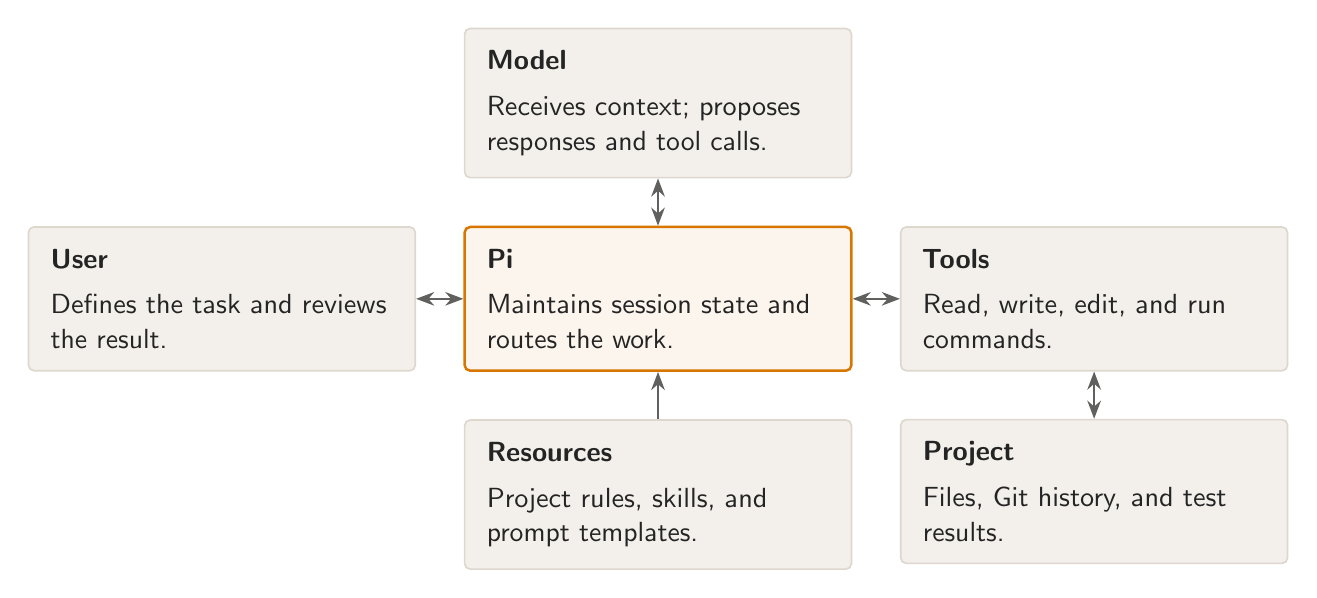
\begin{tikzpicture}
    \node[pihub] (pi) {\pilabel{Pi}{Maintains session state and routes the work.}};
    \node[picard,left=6mm of pi] (user) {\pilabel{User}{Defines the task and reviews the result.}};
    \node[picard,right=6mm of pi] (tools) {\pilabel{Tools}{Read, write, edit, and run commands.}};
    \node[picard,above=6mm of pi] (model) {\pilabel{Model}{Receives context; proposes responses and tool calls.}};
    \node[picard,below=6mm of pi] (resources) {\pilabel{Resources}{Project rules, skills, and prompt templates.}};
    \node[picard,below=6mm of tools] (project) {\pilabel{Project}{Files, Git history, and test results.}};
    \draw[piexchange] (user)--(pi); \draw[piexchange] (pi)--(model);
    \draw[piexchange] (pi)--(tools); \draw[piflow] (resources)--(pi);
    \draw[piexchange] (tools)--(project);
  \end{tikzpicture}\end{pifigure}}
\newcommand{\pifirstsession}{\pifour{01 / Project}{Start in the correct directory.}{02 / Inspect}{Ask for the repository summary and checks.}{03 / Act}{Give one bounded task with acceptance criteria.}{04 / Verify}{Read the tool output, run checks, and inspect the diff.}}
\newcommand{\pitoolmap}{%
  \begin{pifigure}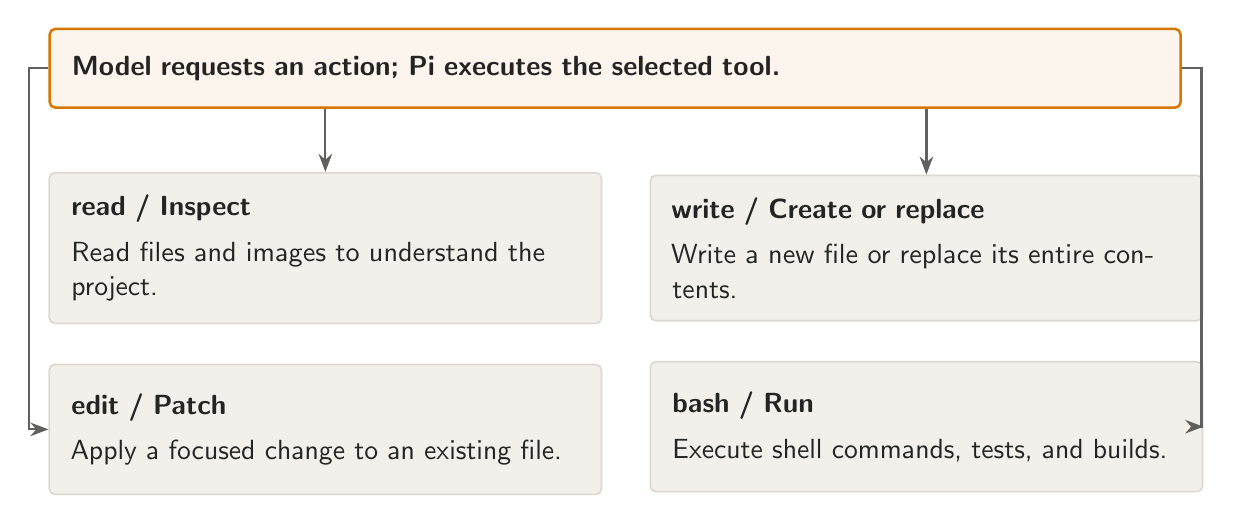
\begin{tikzpicture}
    \node[pihub,text width=13.8cm,minimum height=1cm] (pi) {\textbf{Model requests an action; Pi executes the selected tool.}};
    \node[picard,text width=6.45cm,below=8mm of pi.south west,anchor=north west] (read) {\pilabel{read / Inspect}{Read files and images to understand the project.}};
    \node[picard,text width=6.45cm,right=6mm of read] (write) {\pilabel{write / Create or replace}{Write a new file or replace its entire contents.}};
    \node[picard,text width=6.45cm,below=5mm of read] (edit) {\pilabel{edit / Patch}{Apply a focused change to an existing file.}};
    \node[picard,text width=6.45cm,below=5mm of write] (bash) {\pilabel{bash / Run}{Execute shell commands, tests, and builds.}};
    \draw[piflow] (pi.south -| read.north)--(read.north);
    \draw[piflow] (pi.south -| write.north)--(write.north);
    \draw[piflow] (pi.west)--++(-.25,0)|-(edit.west);
    \draw[piflow] (pi.east)--++(.25,0)|-(bash.east);
  \end{tikzpicture}\end{pifigure}}
\newcommand{\piinspectflow}{\pifour{01 / Locate and understand}{Find entry points, constraints, and tests.}{02 / Plan}{Propose the smallest change; review the scope.}{03 / Change}{Implement the agreed patch.}{04 / Verify}{Run checks and compare the diff with the requirement.}}
\newcommand{\pitrust}{\pithree{Project trust}{Decide whether project resources should load.}{Loaded resources}{Settings, skills, and packages shape behavior.}{Execution boundary}{Tools run with the permissions available to Pi.}}
\newcommand{\pigitcheckpoint}{\pifour{01 / Checkpoint}{Inspect Git status and create a working branch.}{02 / Pi works}{Bound the task and change the relevant files.}{03 / Evidence}{Read the diff and the check results.}{04 / Human decision}{Stage reviewed files; commit what you understand.}}
\newcommand{\pisessions}{%
  \begin{pifigure}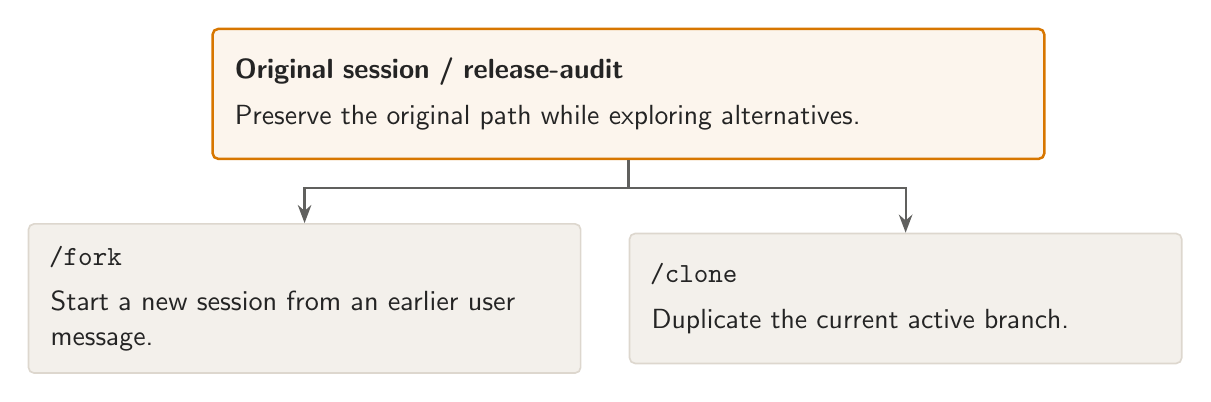
\begin{tikzpicture}
    \node[pihub,text width=10cm] (a) {\pilabel{Original session / release-audit}{Preserve the original path while exploring alternatives.}};
    \node[picard,text width=6.45cm,below left=8mm and -4.7cm of a] (b) {\pilabel{\texttt{/fork}}{Start a new session from an earlier user message.}};
    \node[picard,text width=6.45cm,right=6mm of b] (c) {\pilabel{\texttt{/clone}}{Duplicate the current active branch.}};
    \draw[piflow] (a.south)--++(0,-.35)-|(b.north);
    \draw[piflow] (a.south)--++(0,-.35)-|(c.north);
  \end{tikzpicture}\end{pifigure}}
\newcommand{\picompaction}{\pithree{Active context}{Conversation, tool output, decisions, and open work.}{Compaction}{Summarize older context; retain recent messages.}{Working context}{Continue from the summary and retained messages.}}
\newcommand{\piprintmode}{\pithree{Prompt}{One request, with a read-only tool allowlist in this example.}{Pi / Print mode}{Run the task without an interactive session UI.}{Text output}{Read and validate the response before taking action.}}
\newcommand{\pijsonmode}{\pithree{Pi}{Emit session, message, and tool events.}{JSONL stream}{Assemble deltas by content index.}{Consumer}{Use \texttt{message\_end} as the final message authority.}}
\newcommand{\pioutputmode}[3]{\pithree{Pi / #1}{Headless process.}{Protocol}{#2}{Client}{#3}}
\newcommand{\pistack}{\begingroup\tikzset{piflow/.style={draw=none}}\pifour{Context files}{Keep durable project rules present.}{Skills and prompts}{Load procedures and reuse task instructions.}{Extensions}{Add tools, commands, events, UI, and gates.}{Packages}{Distribute resources through npm, Git, or a local path.}\endgroup}
\newcommand{\pigate}{\pithree{Tool request}{A Bash command is requested.}{Gate}{Inspect the command and request confirmation.}{Decision}{Allow execution or block it with a reason.}}
\newcommand{\pilocalmodel}{\pithree{Pi}{Use the same agent workflow.}{API endpoint}{Route requests to an OpenAI-compatible localhost server.}{Ollama}{Run the model locally.}}
\newcommand{\pisdk}{\pithree{Application}{A Node or TypeScript product.}{SDK session}{Manage state, events, and prompts.}{Pi workflow}{Connect the model, tools, and project.}}
\newcommand{\pisandbox}{\pithree{Host}{Choose which files and credentials to expose.}{Container}{Run Pi with the mounts, credentials, and network provided.}{Boundary}{Writable mounts can still change host files.}}
